
\chapter{Method 1: Direct intersection}
\label{ch:direct_intersection}

The first presented method to extract a triangulated surface from the VML's data model is by directly processing the stored triangles inside the VML's regular grid.
This approach is the most naive, computationally intensive, but, in theory, most accurate.
It is conceptually equivalent to directly intersecting the mesh of the stock with each swept volume mesh.
Boolean operations on triangle meshes are already available in most CAD kernels.
However, these kernels usually require the meshes to be closed.
Due to the triangle elimination strategy using cell classification, \cf section \ref{sec:classification}, the meshes stored in the regular grid are no longer closed.
Thus, regular CAD kernels cannot be used to intersect the meshes maintained by the VML and a custom mesh intersection algorithm has been developed.


\section{Concept}
\label{sec:direct_intersection_concept}

Every time a swept volume is added to the VML, a unique id is generated and assigned to each of the swept volume's triangles before they are mapped to the cells of the regular grid.
As the stock is internally treated as a swept volume, by inverting the surface normals, all stock triangles are also assigned a unique id.
These ids allow to separate the triangles contained in the regular grid into the previous swept volumes, referred to as structures.
Due to the regular grid's classification, \cf section \ref{sec:classification}, triangles might have been removed and, consequently, the structures put together from the regular grid's cells may no longer be closed meshes.
The separated structures are then processed in pairs.
Each pair is united into a new structure.
The union of the two structure meshes is calculated by intersecting each triangle of one mesh with each triangle of the other mesh.
If two triangles intersect, the intersection line is recorded for both triangles.
After intersection, each triangle with intersection lines is split along these lines, retriangulated and replaced by the triangles resulting from the retriangulation.
All previous intersection lines are now edges of new triangles.
Each triangle of one structure is then tested against the other structure, whether the triangle is inside or outside the other structure, \eg by casting a ray from the triangle to the other structure.
As all triangles intersecting the opposite structure have been split, this property should be unambiguously determinable for each triangle.
By removing all triangles inside the opposite structure, the remaining triangles form a new surface which corresponds to the union of both structures.
This new structure is then again pairwise united with other structures until only one structure is left.
This final structure is the reconstructed surface of the VML's data model.

As it turns out, the test whether a triangle is inside another structure may fail if the tested structure is not a closed mesh, a common case.
An example of such an issue is shown in figure \ref{fig:inside_test_error}.
%
\begin{figure}
	\centering
	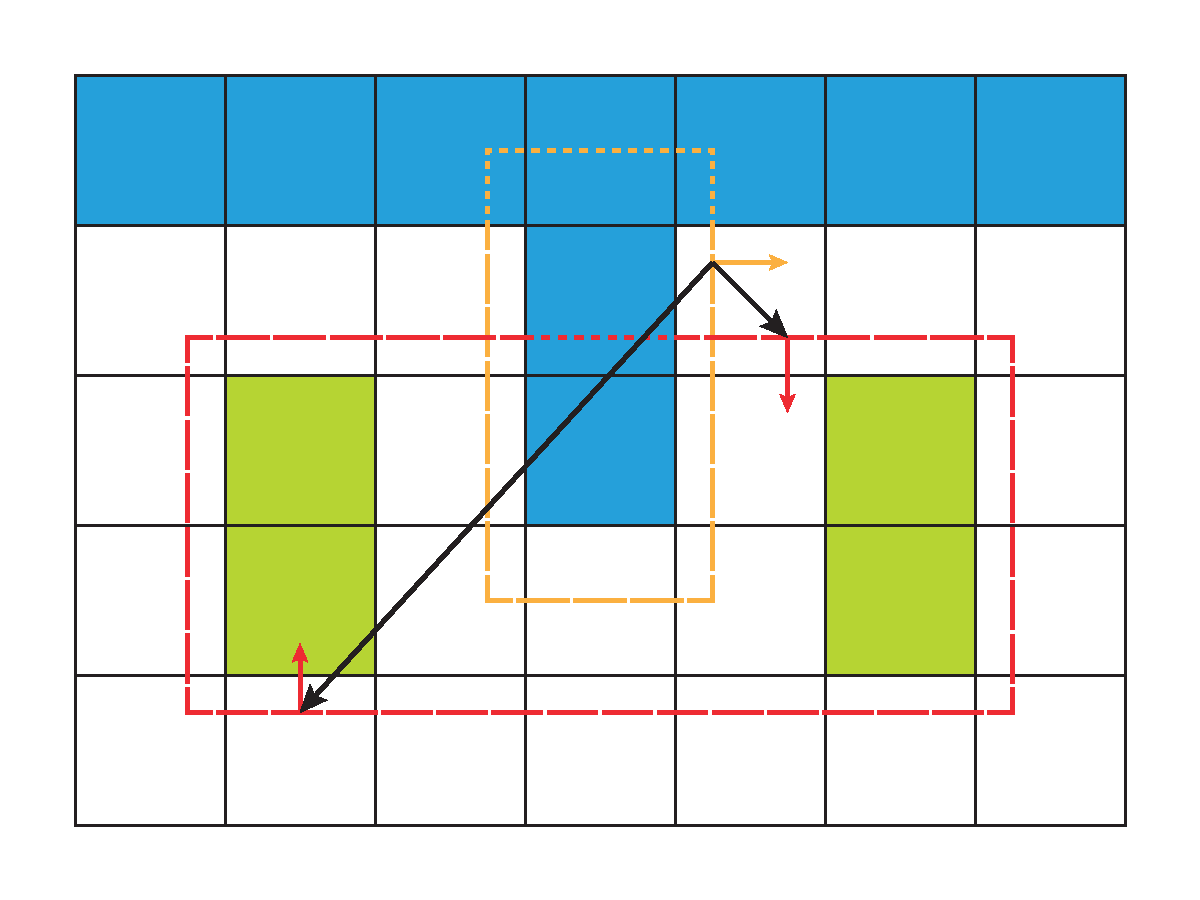
\includegraphics[width=0.8\textwidth]{inside_test_error}
	\caption{
		Testing if a triangle of one structure is inside another structure using a ray.
		Due to triangle elimination, the ray can miss removed structures, \eg when traversing outside cells, causing the inside test to fail, \cf. left ray.
		As structures are guaranteed to be closed within a cell, this test is only valid within a cell, \cf right ray.
	}
	\label{fig:inside_test_error}
\end{figure}
%
A triangle is tested against a structure by using a ray.
This ray is shot from an arbitrary point on the triangle, which does not lie on an edge, \eg the triangle's centroid, to an arbitrary point on a triangle of the other structure.
If the ray does not intersecting the other structure on its way, a comparison of the ray's direction with the normal of the targeted triangle determines whether the ray's origin, the tested triangle, is inside the other structure or not.
However, as classification might eliminate triangles, the ray could potentially intersect triangles of the structure which have been removed, \cf left ray in figure \ref{fig:inside_test_error}.
The regular grid only guarantees closed meshes within a cell.
To circumvent this issue, the inside test for a triangle must be conducted within a cell.

In general, intersecting each triangle of a structure against each other triangle of another structure is an expensive undertaking.
The cost of this operation is $\mathcal{O}(n^2)$, assuming both structures have $n$ triangles.
Intersecting the structures at the level of each cell greatly reduces the value of $n$.
Unfortunately, many triangles usually span the bounding box of a cell and are duplicated in each encompassed cell.
To avoid duplicates or overlapping triangles when combining results from neighboring cells, all triangles of a cell have to be clipped against the cell's bounding box.
This step can be done before intersecting the structures of a cell ....

TODO: check clipping after elimination

Why it does not work on larger meshes?
Run time complexity
Numerical robustness



\section{Implementation}
\label{sec:direct_intersection_implementation}


by testing  


\section{Results}
\label{sec:direct_intersection_results}

